\chapter{Qu'est-ce que la turbulence ? La description hydrodynamique de Kolmogorov}
\renewcommand\partie{\Partie\ Chapitre \thechapter}
\label{ch-01}

%\medskip
\minitoc  

\bigskip


Quand on parle de turbulence, la première image qui résonne dans notre esprit est un écoulement semblant chaotique, des secousses dans un avion ou un enfant qui n'en fait qu'à sa tête. Les propriétés partagées par ces trois exemples sont l'agitation, l'apparent désordre, l'imprévisibilité. Mais ce n'est qu'apparence. Contrairement au pur chaos, ce comportement est statistiquement prévisible et peut montrer un semblant d'ordre.  Dans ce chapitre, sont résumés des notions, notations et outils permettant de caractériser et prédire le comportement d'un écoulement turbulent dans un cadre \ac{HD}. 

\section{Définition et propriétés d'un écoulement turbulent}\label{sec-011}

Supposons l'écoulement incompressible, c'est-à-dire un fluide de densité constante $\rho_0$. L'hypothèse incompressible impose aussi une contrainte sur la vitesse de l'écoulement, le champ vectoriel $\boldsymbol{v}(t,\mathbf{x})$ dépendant du temps $t$ et de la position $\mathbf{x}$, : l'annulation de la divergence de la vitesse, c'est-à-dire, mathématiquement, en notant $\nabla = \frac{\partial}{\partial \mathbf{x}}$, l'opérateur de dérivation spatiale, $\nabla \cdot \boldsymbol{v}  = 0$. 

Un écoulement hydrodynamique incompressible est un système modélisé par les équations de Navier-Stockes incompressibles : 
\begin{eqnarray}
     \label{eq:navst_r} \nabla \cdot \boldsymbol{v} & =& 0 \\
  \label{eq:navst_v}  \partial_t \boldsymbol{v} + \boldsymbol{v} \cdot \nabla \boldsymbol{v} &=& - \frac{1}{\rho_0} \nabla p + \nu \Delta \boldsymbol{v}.
\end{eqnarray}
Le premier terme de l'équation \eqref{eq:navst_v}, $\partial_t \boldsymbol{v}$, indique que cette équation est celle de l'évolution temporelle, $\partial_t = \frac{\partial}{\partial t}$ étant la dérivée partielle temporelle, de la vitesse de l'écoulement $\boldsymbol{v}$. 
Le deuxième terme, $\boldsymbol{v} \cdot \nabla \boldsymbol{v}$, implique un déplacement convectif du champ de vitesse à la vitesse de l'écoulement. Ce terme cristallise les non-linéarités du système. Dimensionnellement, on peut le schématiser par $C_{NL} = \frac{V^2}{L}$ avec $V$ la vitesse caractéristique de l'écoulement et $L$ sa largeur caractéristique. 
Le terme $- \frac{1}{\rho_0} \nabla p $ avec $p$ la pression du fluide dénote les forces de pressions impliquées dans l'écoulement. 
Le dernier terme, $\nu \Delta \boldsymbol{v}$, est un terme dissipatif, d'effort visqueux. Il dépend de $\nu$, la viscosité du fluide, et de $\Delta = \nabla^2$, l'opérateur Laplacien. Ce terme vient contrebalancer le terme convectif et, s'il domine, rend l'écoulement laminaire. On peut le schématiser tel que $C_{D} = \nu \frac{V}{L^2}$. 

Le rapport entre $C_{NL}$ et $C_D$ est le nombre de Reynolds $R_e = \frac{C_{NL}}{C_D} = \frac{VL}{\nu}$, un nombre sans dimension caractérisant le régime de l'écoulement, laminaire ($R_e$ faible) ou turbulent ($R_e \gg 1$). Ces régimes sont illustrés sur la \figref{fig:ecoulement}. Dans cette expérience, un jet d'eau (blanc) est injecté dans de l'eau stagnante (espace noir). À gauche, sa largeur caractéristique est imposée par le diamètre du tuyau d'injection, l'écoulement est alors dans un régime laminaire. Ensuite la turbulence se développe (régime transitoire), il y a apparition de tourbillons (vortex) dans l'écoulement. Enfin, tout à droite, la turbulence est pleinement développée, les non-linéarités dominent et s'entretiennent. 
\begin{figure}[!ht]
 \centering
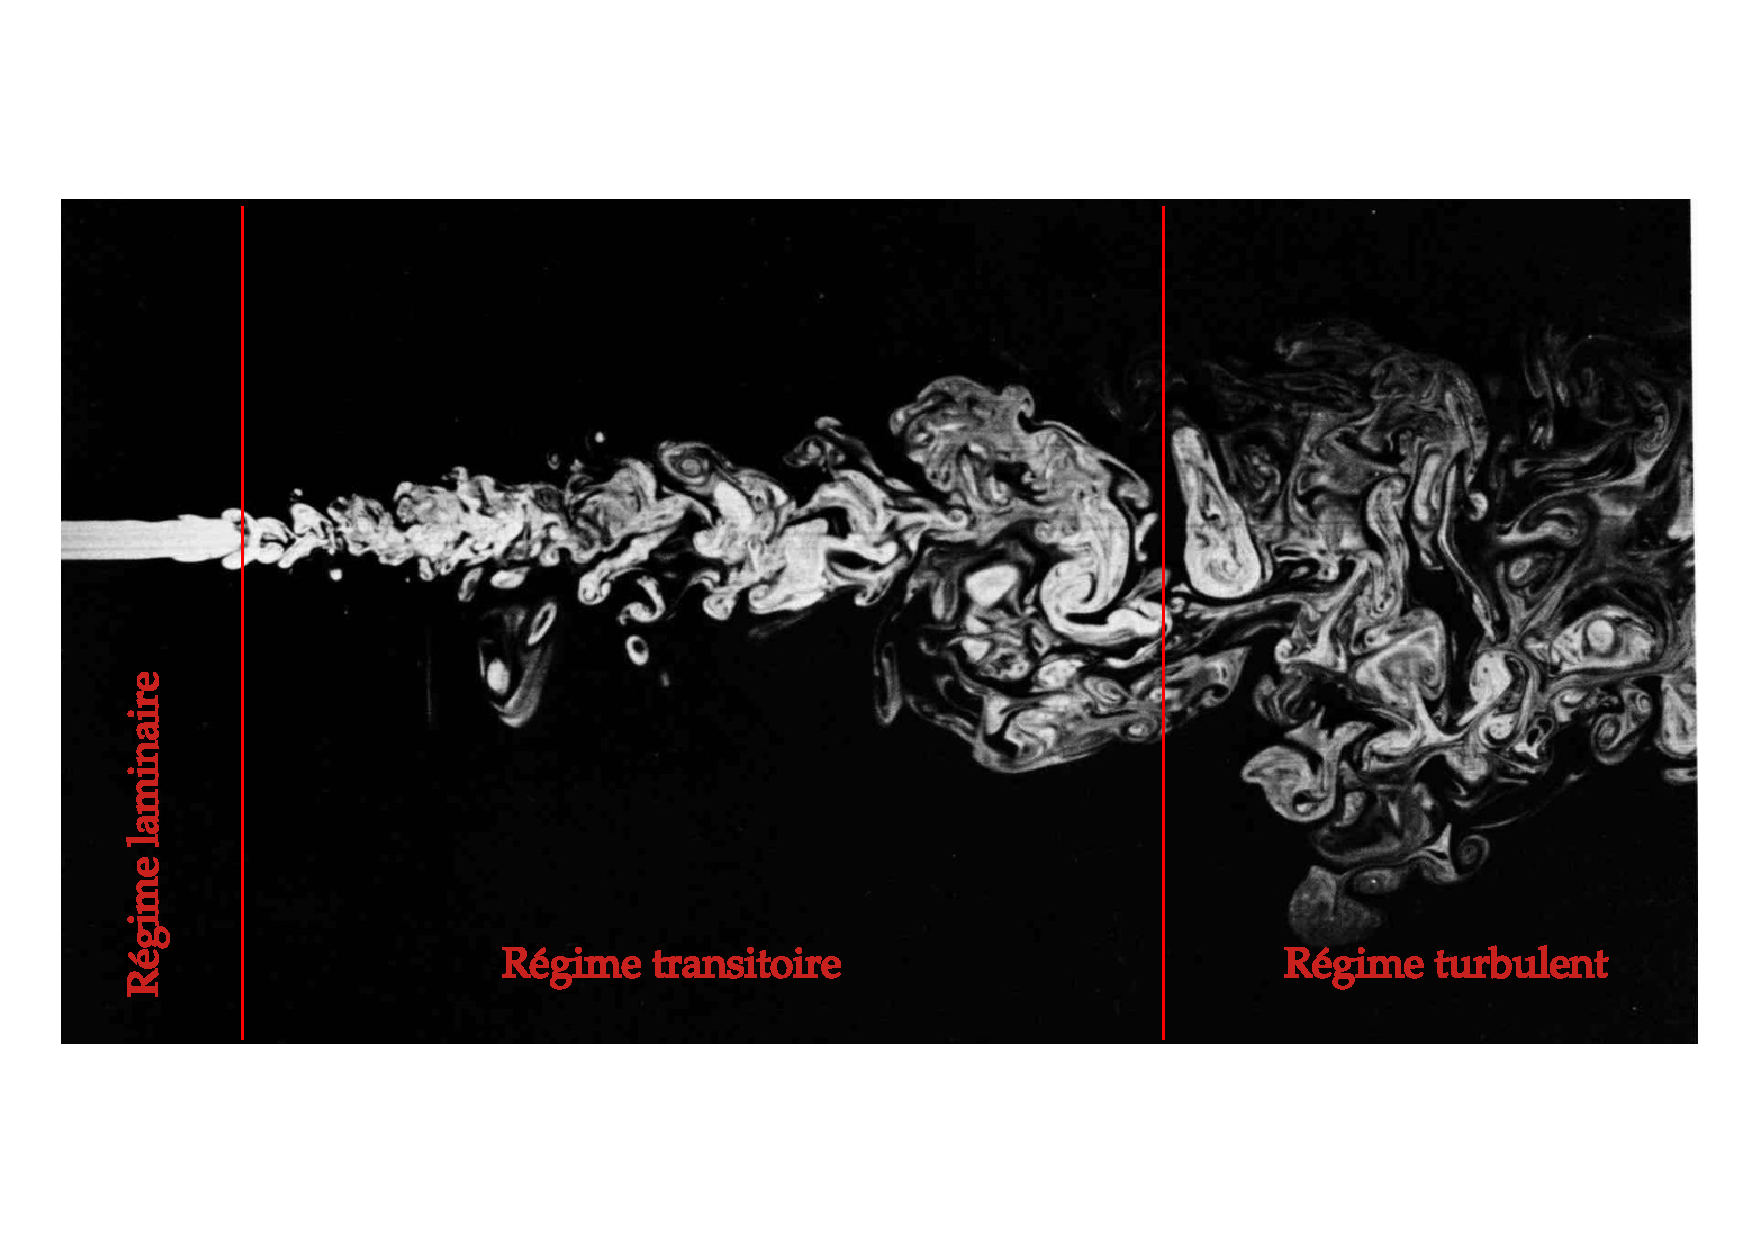
\includegraphics[width=\linewidth,trim=1cm 3cm 1cm 3cm, clip=true]{./Part_0/images/turbul_Re}
\cprotect\caption{Injection d'un jet d'eau dans de l'eau observée par fluorescence laser et illustrant les différents régimes d'un écoulement : laminaire, transitoire et turbulent. Crédits de l'image initiale : [\cite{van_dyke_album_1982}].}
\label{fig:ecoulement}
\end{figure}

Dans le cadre hydrodynamique incompressible, l'écoulement n'est décrit que par les champs de vitesse et de pression mais pour d'autres fluides, la description peut impliquer d'autres champs tels que le champ magnétique $\boldsymbol{B}$, le champ scalaire massique $\rho$, etc. On peut définir un nombre sans dimension similaire au nombre de Reynolds, rapport entre le terme non-linéaire convectif et le terme diffusif ou dissipatif impliqués dans l'évolution temporelle de ces champs. Dans le cas d'un champ magnétique, ce sera le nombre de Reynolds magnétique $R_m = \frac{VL}{\eta}$ avec $\eta$ la résistivité ou diffusivité magnétique. Pour des quantités thermodynamiques telles que la densité de masse, la pression, etc., on parlera plutôt de nombres de Péclet.

 Sur la \figref{fig:comp_turbul}, sont présentés des résultats d'une simulation turbulente tridimensionnelle qui sera introduite et utilisée dans la partie \ref{part_3}. 
\begin{figure}[!ht]
 \centering
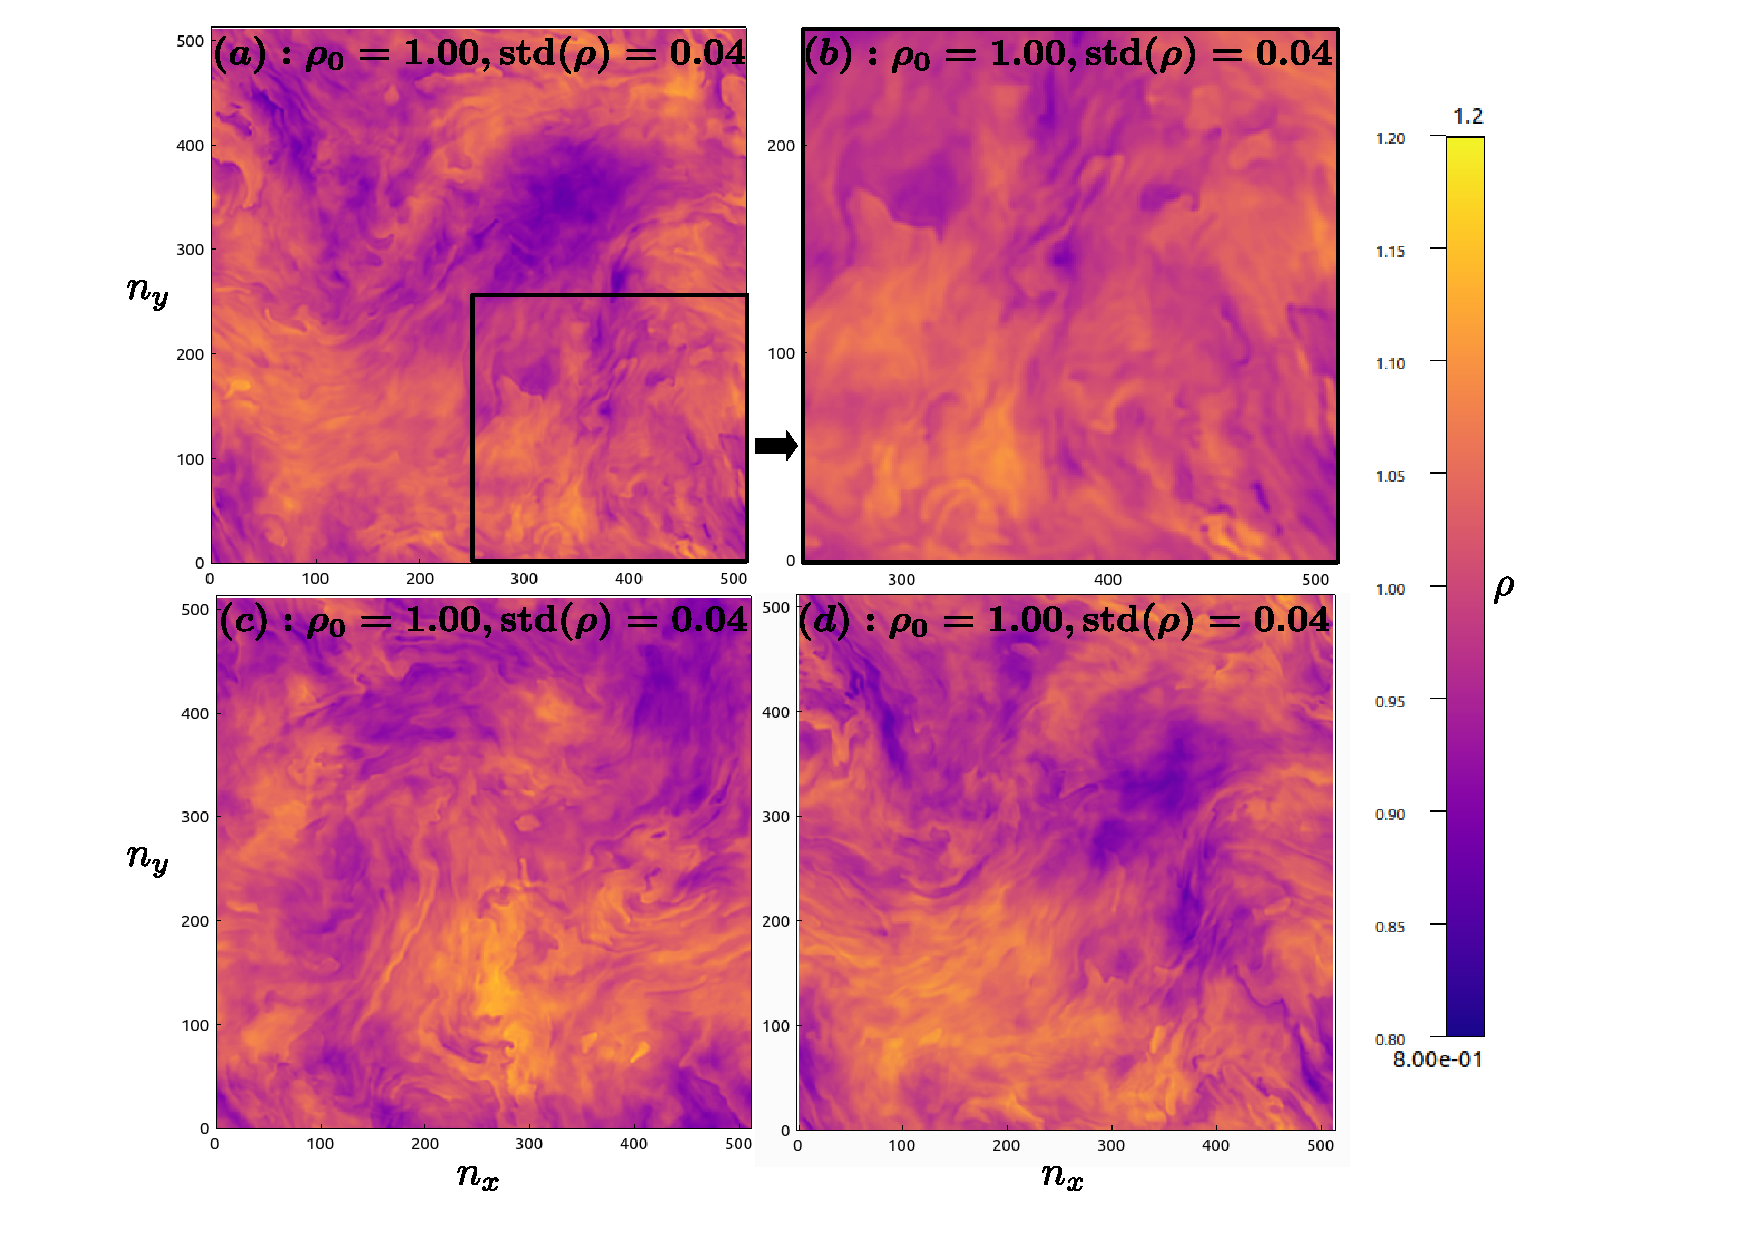
\includegraphics[width=0.8\linewidth,trim=2cm 0cm 4cm 0cm, clip=true]{./Part_0/images/simu_panel_rho}
\cprotect\caption{Résultats d'une simulation 3D d'un plasma turbulent décrit par le modèle Hall-CGL. Le code de simulation sera introduit dans la partie \ref{part_3}). La quantité représentée est la densité $\rho$. Chaque image correspond à une coupe $x-y$ du cube obtenu au temps $t$ (en unité de temps de la simulation). Les axes sont en position numérique (nombre de points dans chaque direction, comptés à partir d'une position $(0,0,0)$). (a) : $n_z=323$, $t=410$. (b) : zoom de (a). (c) : $n_z=638$, $t=410$. (d) : $n_z=323$, $t=408$. Pour chaque image, la moyenne spatiale, $\rho_0$, est de $\num{1.00}$ et l'écart-type, $\text{std}(\rho)$, de $\num{0.04}$.}
\label{fig:comp_turbul}
\end{figure}
L'image (a) correspond à une coupe du cube de densité $\rho$ telle que $n_z=323$ obtenue au temps $t=410$. Si on la compare à l'image (c) (autre coupe du même cube telle que $n_z=638$), on remarque une certaine invariance spatiale statistique qui illustre la propriété d'homogénéité dite statistique d'un fluide turbulent. Si par contre, on la compare à l'image (d) (coupe $n_z=323$ obtenue à la date $t=408$), on retrouve similairement une certaine invariance temporelle qui vient illustrer la propriété de stationnarité statistique du fluide. Et, en comparant avec l'image (b) (un zoom de l'image (a)), on observe ce qui semble être une loi d'échelle. 

Un écoulement ou un fluide turbulent serait donc caractérisé par 
\begin{itemize}
    \item une dominance des non-linéarités sur les contributions diffusives (grands nombres de Reynolds et de Péclet),
    \item des propriétés d'invariance (homogénéité, stationnarité) au sens statistique,
    \item une loi d'échelle.
\end{itemize}
Dans la section \ref{sec-012}, on va définir les notations et appellations liées aux notions mathématiques statistiques et dans la section \ref{sec-013}, on abordera un peu plus en détail la description de la turbulence à travers les échelles.

\section{Description statistique et notations pour l'étude d'un système turbulent}\label{sec-012}

Afin de garder la description du travail présenté dans ce mémoire accessible à tous, nous ne nous perdrons pas dans des définitions mathématiques complexes et exhaustives des notions, mais resterons sur des définitions exemplifiées et plus appliquées. 

Dans l'ensemble de ce mémoire, on se placera dans le cadre tridimensionnel (3D). Sauf quantités indéfinies, les grandeurs vectorielles seront notées en gras. Le système de représentation spatial sera génériquement cartésien $\mathbf{x} = (x,y,z)$, sauf mention contraire.

Soit une quantité indéfinie $X$ (densité, vitesse, pression, champ magnétique, etc.) caractérisant un fluide. La distribution de valeurs possibles pour $X$, ou distribution de probabilité de $X$, notée $\mathcal{P}_X$, peut être obtenue en considérant différents points de vue :
\begin{itemize}
    \item PV1 : Décrire le fluide comme un ensemble souvent discret, par exemple de $N$ particules (atomes, molécules, etc.) associées individuellement à une valeur de la quantité $X$, notée $X_n$ avec $n \in [1;N]$. 
    \item PV2 : Regarder l'espace occupé par le fluide : un volume continu $V$ ou un nombre de points d'emplacement $\mathbf{x}$. La quantité $X$ sera alors évaluée en chacun d'eux et notée $X(\mathbf{x})$. 
    \item PV3 : Ne considérer qu'une particule ou qu'un point, regarder les valeurs de $X$ au fil du temps sur une période $T$, et les noter $X(t)$. 
\end{itemize}
Ces différents points de vue ne sont pas forcément équivalents. Par exemple, si l'on regarde plusieurs types de particules et que les valeurs de $X$ dépendent de leur nature, ne regarder qu'une particule au fil du temps ne sera pas représentatif du système. Par la suite, on utilisera les représentations PV2 et PV3.  

Pour caractériser la distribution de probabilité de $X$, on peut utiliser divers outils statistiques. L'un d'eux est la moyenne (moment d'ordre 0), une opération linéaire que l'on va noter $\left<X\right>$ et qui est définie en fonction des points de vue :
\begin{itemize}
    \item PV1 : $\left<X\right>_{N} = \frac{1}{N} \sum_{n=1}^N X_n$, est la moyenne d'ensemble définie de manière discrète.
    \item PV2 : $\left<X\right>_{V} = \frac{1}{V} \int_V X(\mathbf{x}) \mathcal{P}_X d\mathbf{x}$, est la définition continue de la moyenne spatiale. $\left<X\right>_V$ est indépendante de la position locale $\mathbf{x}$. Dans le cas discret, en considérant un échantillonnage spatial, c'est-à-dire $N_V$ points dans le volume $V$, et en notant $X_p$ la valeur de $X$ au point $p$, $\left<X\right>_{V} = \frac{1}{N_V} \sum_{p=1}^{N_V} X_p$. 
    \item PV3 : $\left<X\right>_{T} = \frac{1}{T} \int_0^T X(t) \mathcal{P}_X dt$, est la définition continue de la moyenne temporelle. $\left<X\right>_T$ est indépendant de l'instant $t$. Une moyenne discrète peut aussi être définie en considérant un échantillonnage temporel.
\end{itemize}
Si $\left<X\right>_{N} = \left<X\right>_{V} = \left<X\right>_{T}$, on peut supposer une équivalence statistique des différents points de vue. Le système sera alors ergodique. 

On peut définir plus rigoureusement les propriétés d'homogénéité et de stationnarité statistiques à l'aide de $\mathcal{P}_X$ : 
\begin{itemize}
    \item \textbf{\emph{homogénéité statistique}} : soient deux échantillons représentatifs du système et définis relativement à deux positions indépendantes l'une de l'autre $\mathbf{x}$ et $\mathbf{x'}$ alors  $\mathcal{P}_X(\mathbf{x}) = \mathcal{P}_X(\mathbf{x'}) = \mathcal{P}_X$, ce qui implique pour la moyenne $\left<X(\mathbf{x})\right> = \left<X(\mathbf{x'})\right> = \left<X\right>$,
    \item \textbf{\emph{stationnarité statistique}} : soient deux échantillons représentatifs du système et définis relativement à deux instants indépendants l'un de l'autre $t$ et $t'$ alors $\mathcal{P}_X(t) = \mathcal{P}_X(t') = \mathcal{P}_X$, ce qui implique pour la moyenne $\left<X(t)\right> = \left<X(t')\right> = \left<X\right>$.
\end{itemize}
Attention, cela ne signifie pas que localement, entre deux instants $t$ ou deux positions $\mathbf{x}$, $X$ sera constant. En pratique, dans des données d'observations ou de simulations, des échantillons dans lesquels ces hypothèses seraient parfaitement valides sont difficiles à obtenir. Des compromis devront donc être établis. 

Similairement aux définitions des propriétés d'homogénéité et de stationnarité statistiques, pour étudier un fluide turbulent, on doit relier le comportement statistique de deux échantillons ou plus, c'est-à-dire que l'on doit s'intéresser aux fluctuations, incréments de quantités et corrélations entre au moins deux échantillons. Ce lien peut s'exprimer en fonction de la distance temporelle ou spatiale entre ces échantillons, généralement appelée <<échelle>>. En 1941, Kolmogorov pose les bases d'une théorie permettant d'obtenir une telle relation : la théorie des lois exactes [\cite{frisch_turbulence_1995,kolmogorov_local_1991,kolmogorov_dissipation_1991}]. Cette théorie repose sur les hypothèses que nous avons illustrées dans la section \ref{sec-011} (dominance des effets non-linéaires, homogénéité et stationnarité statistiques) ainsi que sur une hypothèse plus spécifique de séparation d'échelle qui sera expliquée dans la section \ref{sec-013}.

Le travail décrit dans ce mémoire est basé sur cette théorie et implique les notations suivantes. On considèrera deux échantillons définis relativement à deux positions\footnote{Il est possible de corréler plus de deux points. Tout lecteur intéressé pourra se référer à [\cite{cho_simulations_2009}].}\footnote{Historiquement, les calculs sont effectués dans le cadre PV2. Il serait a priori possible de les transposer dans les cadres PV1 ou PV3, mais ce n'est pas l'objet de cette thèse.} indépendantes l'une de l'autre, $\mathbf{x}$ et $\mathbf{x'}$. La quantité indéfinie $X$ évaluée en $\mathbf{x'}$ sera notée $X'$ et celle évaluée en $\mathbf{x}$, $X$. L'échelle, notée $\boldsymbol{\ell}$, sera définie comme l'incrément de position : 
\begin{equation}
    \boldsymbol{\ell} = \delta \mathbf{x} = \mathbf{x'} - \mathbf{x} ,
\end{equation}
avec $\delta$ dénotant le caractère incrémental de la quantité (ici la position). L'incrément de la quantité indéfinie $X$ s'écrirait : 
\begin{equation}
    \delta X = X' - X = X(\mathbf{x'}) - X(\mathbf{x})  .
\end{equation}

Le lien étudié entre les deux échantillons sera une fonction de corrélation spatiale entre deux quantités $X$ et $Y$ (ici indéfinies) qui s'obtient en considérant une quantité au point $\mathbf{x}$ et l'autre au point $\mathbf{x'}$, en les multipliant puis en moyennant. Afin de conserver une symétrie du rôle de $\mathbf{x}$ et $\mathbf{x'}$, on définira la fonction de corrélation telle que 
\begin{equation}
    \label{eq:def_correlation} \mathcal{R}_{XY} = \frac{1}{2} \left<X \cdot Y' + X' \cdot Y\right>,
\end{equation}
en notant $\cdot$ l'opération générique multiplicative. Entre deux vecteurs, cette opération pourrait être considérée comme un produit scalaire ou remplacée par un produit vectoriel noté $\times$. La fonction d'auto-corrélation est obtenue en considérant $X=Y$, c.-à-d. $\mathcal{R}_{XX} = \left<X \cdot X'\right>$. 
La moyenne $\left<\right>$ impliquée dans ces fonctions est la moyenne spatiale. $\mathcal{R}_{XY}$ sera donc indépendant de $\mathbf{x}$ et $\mathbf{x'}$ et ne dépendra que de $\boldsymbol{\ell}$ et a priori de $t$ si les quantités dépendent du temps. 

Par indépendance entre le temps et la position, la moyenne spatiale commute avec la dérivée temporelle : 
\begin{equation}
  \label{eq:prop_t}  \partial_t \left<X\right> = \left<\partial_t X\right> .
\end{equation}
On note  $\nabla_{\boldsymbol{\ell}} = \frac{\partial}{\partial \boldsymbol{\ell}}$ l'opérateur de dérivation spatiale dans l'espace global des échelles, $\nabla$ et $\nabla'$ les opérateurs de dérivation locaux respectivement en $\mathbf{x}$ et $\mathbf{x'}$. L'indépendance entre $\mathbf{x}$ et $\mathbf{x'}$, implique que :
\begin{equation}
  \label{eq:prop_x}    \nabla X' = 0,  \qquad \nabla' X = 0.
\end{equation}
Grâce à l'hypothèse d'homogénéité statistique, ces opérateurs dérivatifs vérifient\footnote{
Soient $A$, $B$ et $C$ des quantités indéfinies telles que $A(\boldsymbol{\ell}) = \left<B \cdot C'\right> = \left<B(\mathbf{x}) \cdot C(\mathbf{x'})\right>$  avec $\cdot$ une opération multiplicative quelconque et $\mathbf{x'} = \mathbf{x} + \boldsymbol{\ell}$. Alors, l'élément différentiel $d \boldsymbol{\ell} $ est égal à $d \mathbf{x'} - d \mathbf{x}$. 

À $\mathbf{x}$ fixé, $ d \boldsymbol{\ell} = d \mathbf{x'}$, alors
$\nabla_{\boldsymbol{\ell}} A(\boldsymbol{\ell}) = \left<\partial_{\boldsymbol{\ell}} (B \cdot  C')\right> = \left<\partial_{\mathbf{x'}} (B \cdot  C') \right> = \left<\nabla' (B \cdot  C')\right> $. D'où la relation entre les opérateurs :  $\nabla_{\boldsymbol{\ell}} \left<\right> = \left<\nabla'\right>$. Similairement, à $\mathbf{x'}$ fixé, $ d \boldsymbol{\ell} = - d \mathbf{x}$, d'où $\nabla_{\boldsymbol{\ell}} \left<\right> = - \left<\nabla\right>$.
}
\begin{equation}
   \label{eq:prop_l}   \nabla_{\boldsymbol{\ell}}\left<\right> = \left<\nabla' \right> = - \left<\nabla \right> .
\end{equation}

En turbulence, on utilise aussi communément la transformée de Fourier. Cette méthode permet de travailler dans un espace où la position est repérée par $\boldsymbol{k} \propto 1/\mathbf{x}$, et où toute quantité se retrouve décomposée en une série de <<modes>> que l'on appelle un spectre. Dans le cas continu 3D, on définit la transformée de Fourier de la quantité $X$ par 
\begin{equation}
    \tilde{X}(\boldsymbol{k}) = \frac{1}{(2\pi)^3} \iiint X(\mathbf{x}) e^{-i\boldsymbol{k} \cdot \mathbf{x}} d\mathbf{x}
\end{equation}
et la transformée inverse par 
\begin{equation}
    X(\mathbf{x}) = \iiint \tilde{X}(\boldsymbol{k}) e^{i\boldsymbol{k} \cdot \mathbf{x}} d\boldsymbol{k}.
\end{equation} 
On remarque qu'en termes de dimensions, si l'on note $[X]$ l'unité de $X$ et $L$ l'unité de longueur, $\tilde{X} \sim [X] L^3$.

Dans le cas continu 1D, on aura similairement : 
\begin{equation}
    \tilde{X}(k) = \frac{1}{2\pi} \int X(x) e^{-ikx} dx , \qquad 
    X(x) = \int \tilde{X}(k) e^{ikx} dk
\end{equation} 
et en termes de dimensions, $\tilde{X} \sim [X] L$.

Ces notations et hypothèses seront utilisées tout au long de ce mémoire. Pour se familiariser avec leur utilisation, une application de la théorie de Kolmogorov à un écoulement hydrodynamique incompressible décrit par les équations de Navier-Stockes \eqref{eq:navst_r} et \eqref{eq:navst_v} est donnée dans la section \ref{sec-013}. Cette application va nous servir à introduire la notion de loi d'échelle et l'hypothèse de séparation d'échelle.


\section{Théorie de Kolmogorov et loi d'échelle}\label{sec-013}

La démonstration de Kolmogorov de 1941 [version traduite :  \cite{kolmogorov_local_1991,kolmogorov_dissipation_1991}] a été réécrite à de multiples reprises sous différentes formes. D'autres versions sont données par \cite{monin_statistical_1975}, \cite{frisch_turbulence_1995}, \cite{antonia_analogy_1997}, et \cite{galtier_physique_2021}. 

Pour faciliter les étapes de calcul, on va réécrire l'équation de Navier-Stockes \eqref{eq:navst_v} grâce à l'hypothèse incompressible \eqref{eq:navst_r} et y ajouter un terme de forçage $\boldsymbol{f_c}$ : 
\begin{equation}
  \label{eq:navst_v2}  \partial_t \boldsymbol{v} = - \nabla \cdot (\boldsymbol{v} \boldsymbol{v}) -  \frac{1}{\rho_0} \nabla p + \nu \Delta \boldsymbol{v} + \boldsymbol{f_c} 
.\end{equation}

La démonstration se base sur la recherche d'une équation d'évolution temporelle pour la fonction d'auto-corrélation $\mathcal{R}_{\boldsymbol{v}\boldsymbol{v}} = \left<\boldsymbol{v} \cdot \boldsymbol{v'}\right>$. Pour l'obtenir, on dérive temporellement $\mathcal{R}_{\boldsymbol{v}\boldsymbol{v}}$ grâce à la propriété \eqref{eq:prop_t} (étape \eqref{eq:step_1}), on injecte l'équation de Navier-Stockes \eqref{eq:navst_v2} (étape \eqref{eq:step_2}) puis on applique les propriétés \eqref{eq:prop_x} et \eqref{eq:prop_l} pour extraire les opérateurs dérivatifs spatiaux de la moyenne spatiale (étape \eqref{eq:step_3}) : 
\begin{eqnarray}
    \partial_t \mathcal{R}_{\boldsymbol{v}\boldsymbol{v}} &=& \left<\boldsymbol{v} \cdot \partial_t \boldsymbol{v'} + \boldsymbol{v'} \cdot \partial_t \boldsymbol{v}\right> \label{eq:step_1} \\ 
    &=& - \left< \nabla' \cdot (\boldsymbol{v'} \boldsymbol{v'}) \cdot \boldsymbol{v}   +  \nabla \cdot (\boldsymbol{v} \boldsymbol{v})\cdot\boldsymbol{v'} \right> - \frac{1}{\rho_0} \left<\boldsymbol{v} \cdot \nabla' P' + \boldsymbol{v'} \cdot \nabla P\right>  \nonumber \\
    && + \nu \left<\boldsymbol{v} \cdot \Delta' \boldsymbol{v'} + \boldsymbol{v'} \cdot \Delta \boldsymbol{v}\right> + \left<\boldsymbol{v} \cdot \boldsymbol{f'_c} + \boldsymbol{v'} \cdot \boldsymbol{f_c}\right> \label{eq:step_2} \\  
    &=& \nabla_{\boldsymbol{\ell}} \cdot \left< - \boldsymbol{v} \cdot \boldsymbol{v'} \boldsymbol{v'} + \boldsymbol{v'} \cdot \boldsymbol{v} \boldsymbol{v}\right>  + \frac{1}{\rho_0} \nabla_{\boldsymbol{\ell}} \cdot \left< - P' \boldsymbol{v} + P \boldsymbol{v'}\right> \nonumber \\
    && + 2 \nu \Delta_{\boldsymbol{\ell}} \left<\boldsymbol{v} \cdot \boldsymbol{v'} \right>  + \left<\boldsymbol{v} \cdot \boldsymbol{f'_c} + \boldsymbol{v'} \cdot \boldsymbol{f_c}\right>  \label{eq:step_3}  
.\end{eqnarray}
Avec l'hypothèse incompressible et celle d'homogénéité statistique (propriétés \eqref{eq:prop_x} et \eqref{eq:prop_l}), 
\begin{eqnarray}
    \nabla_{\boldsymbol{\ell}} \cdot \left< - P' \boldsymbol{v} + P \boldsymbol{v'}\right> &=& 0, \\
    \nabla_{\boldsymbol{\ell}} \cdot \left< - \boldsymbol{v} \cdot \boldsymbol{v'} \boldsymbol{v'} + \boldsymbol{v'} \cdot \boldsymbol{v} \boldsymbol{v}\right> &=& \frac{1}{2} \nabla_{\boldsymbol{\ell}} \cdot \left< \delta \boldsymbol{v} \cdot \delta \boldsymbol{v} \delta \boldsymbol{v} \right>, \\
    \left<\boldsymbol{v} \cdot \boldsymbol{f'_c} + \boldsymbol{v'} \cdot \boldsymbol{f_c}\right> &=& \left<\boldsymbol{v} \cdot \left(\boldsymbol{f_c}\left(\mathbf{x}+\boldsymbol{\ell}\right) +  \boldsymbol{f_c}\left(\mathbf{x}-\boldsymbol{\ell}\right)\right)\right>
.\end{eqnarray}

D'où l'équation dite de K\'arm\'an-Howarth-Monin (\acs{KHM}): 
\begin{equation}
    - \frac{\rho_0}{2} \partial_t \mathcal{R}_{\boldsymbol{v}\boldsymbol{v}} + \nu \rho_0 \Delta_{\boldsymbol{\ell}} \mathcal{R}_{\boldsymbol{v}\boldsymbol{v}} + \frac{\rho_0}{2} \left<\boldsymbol{v} \cdot \left(\boldsymbol{f_c}\left(\mathbf{x}+\boldsymbol{\ell}\right) +  \boldsymbol{f_c}\left(\mathbf{x}-\boldsymbol{\ell}\right)\right)\right> = - \frac{\rho_0}{4} \nabla_{\boldsymbol{\ell}} \cdot \left<\delta \boldsymbol{v} \cdot \delta \boldsymbol{v} \delta \boldsymbol{v}\right> \label{eq:KHM_HD}  
.\end{equation} 

Schématiquement, on va la noter : 
\begin{equation}
    \label{eq:bal_KHM} -\partial_t \mathcal{R} + \varepsilon_{NL} + \varepsilon_{F} + \varepsilon_{D} = 0 .
\end{equation} 
\begin{itemize}
    \item $\mathcal{R} = \frac{\rho_0}{2} \mathcal{R}_{\boldsymbol{v}\boldsymbol{v}}$, la fonction de corrélation de densité d'énergie totale (ici cinétique). En $\boldsymbol{\ell} = 0$, elle est égale à la densité d'énergie totale moyenne $\left<\frac{\boldsymbol{v}^2}{2}\right>$ du système.
    \item $\varepsilon_{NL} = \frac{1}{4} \rho_0 \nabla_{\boldsymbol{\ell}} \cdot \left<\delta \boldsymbol{v} \cdot \delta \boldsymbol{v} \delta \boldsymbol{v}\right>$, le taux de cascade ou de transfert non-linéaire de l'énergie incrémentale $\frac{1}{4} \rho_0 \left<\delta \boldsymbol{v}^2\right>$ à travers les échelles, il s'annule en $\boldsymbol{\ell} = 0$.
    \item $\varepsilon_{F} = \frac{1}{2} \rho_0 \left<\boldsymbol{v} \cdot \left(\boldsymbol{f_c}\left(\mathbf{x}+\boldsymbol{\ell}\right) +  \boldsymbol{f_c}\left(\mathbf{x}-\boldsymbol{\ell}\right)\right)\right>$, le taux de forçage dépendant des échelles. En $\boldsymbol{\ell} = 0$, il est égal à la densité d'énergie moyenne injectée $\rho_0 \left<\boldsymbol{v} \cdot  \boldsymbol{f_c}\right>$ dans le système par le forçage.
    \item $\varepsilon_{D} = \rho_0 \nu \Delta_{\boldsymbol{\ell}} \mathcal{R}_{\boldsymbol{v}\boldsymbol{v}}$, le taux de dissipation dépendant des échelles. En $\boldsymbol{\ell} = 0$, il est égal à la densité d'énergie moyenne dissipée par viscosité $\rho_0 \nu \left<\Delta \boldsymbol{v}^2\right>$.
\end{itemize}

On remarque qu'en $\boldsymbol{\ell} = 0$, \eqref{eq:KHM_HD} devient l'équation d'énergie totale moyenne que l'on peut noter : 
\begin{equation}
     \label{eq:bal_KHM0} -  \partial_t \mathcal{R}(\boldsymbol{\ell} =0)  + \varepsilon_{D}(\boldsymbol{\ell} =0) +  \varepsilon_{F}(\boldsymbol{\ell} =0) = 0  
.\end{equation} 

L'hypothèse de stationnarité statistique vient annuler toute dérivée temporelle de quantités moyennées. Par conséquent, les équations \eqref{eq:bal_KHM} et \eqref{eq:bal_KHM0} deviennent :  
\begin{eqnarray}
    \label{eq:bal_eps}\varepsilon_{NL} + \varepsilon_{F} + \varepsilon_{D} &=& 0 ,\\
    \label{eq:bal_eps0} \varepsilon_{D}(\boldsymbol{\ell} =0) +  \varepsilon_{F}(\boldsymbol{\ell} =0) &=& 0
.\end{eqnarray}


Les démonstrations existantes divergent dans le traitement des taux $\varepsilon_{F}$ et $\varepsilon_{D}$ de l'équation \eqref{eq:bal_eps} car elles ne prennent pas forcément en compte $\varepsilon_{F}$. Mais, toutes utilisent une propriété fondamentale de la turbulence, la loi <<zéroième>>. Cette loi indique que, pour un nombre de Reynolds grand, lorsque $\nu$ tend vers 0, la densité d'énergie dissipée moyenne $\rho_0 \nu  \left<\Delta\boldsymbol{v}^2\right>$, qui correspond à  $\varepsilon_D$ évalué en $\boldsymbol{\ell} =0$, devient indépendante de $\nu$ et ne s'annule pas. Cette singularité est aussi appelée anomalie dissipative. Elle indique la présence d'une dissipation dans la limite $R_e \gg 1$. On va noter $-\varepsilon$ cette valeur particulière de  $\varepsilon_D$. On peut alors résumer cette loi comme suit : 
\begin{equation}
 \label{eq:zero}  \varepsilon_D  \xrightarrow[\nu \rightarrow 0]{} \left\{
    \begin{split}
    & 0 & \textrm{si $\boldsymbol{\ell} \neq 0$ } \\
& - \varepsilon &  \textrm{si $\boldsymbol{\ell} =0$ } 
\end{split}
\right.
\end{equation}

Si l'on prend en compte le terme de forçage, il sera supposé actif aux grandes échelles, notées $\boldsymbol{\ell_F} $. Aux échelles $\boldsymbol{\ell} \ll \boldsymbol{\ell_F}$, on obtient\footnote{Une démonstration de cette approximation est donnée dans l'Annexe \ref{an:forc} pour un forçage de type distribution de Dirac dans l'espace de Fourier.} $\varepsilon_{F} = \varepsilon_{F}(\boldsymbol{\ell} =0)$.  Avec la relation \eqref{eq:bal_eps0} et la loi zéroième \eqref{eq:zero}, on obtient alors $\varepsilon_{F}(\boldsymbol{\ell} \ll \boldsymbol{\ell_F}) = \varepsilon$. Enfin, en se plaçant à des échelles différentes de $\boldsymbol{\ell} =0$, telles que $\varepsilon_{D}=0$, on obtient de \eqref{eq:bal_eps}, la loi exacte de Kolmogorov (version dérivée, notée \acs{K41} ) : 
\begin{equation}
 \label{eq:led_kolm} \frac{\varepsilon}{\rho_0} = - \frac{1}{4} \nabla_{\boldsymbol{\ell}} \cdot \left<\delta \boldsymbol{v} \cdot \delta \boldsymbol{v} \delta \boldsymbol{v}\right>
\end{equation}
qui s'écrit schématiquement $\varepsilon=-\varepsilon_{NL}$. Dans ce mémoire, nous déterminerons et analyserons $\varepsilon_{NL}$ pour différents modèles. Si l'on ne prend pas en compte le terme de forçage, on peut construire la différence entre \eqref{eq:bal_KHM} et \eqref{eq:bal_KHM0} et, dans la limite des grands nombres de Reynolds et avec l'hypothèse de stationnarité statistique, on peut retrouver \eqref{eq:led_kolm} [\cite{antonia_analogy_1997}]. 

Cette loi est valable dans une gamme d'échelle dite inertielle où le comportement du fluide est supposé complètement non-linéaire ($R_e \gg 1$ et $\nu \rightarrow 0$) et peu impacté par tout phénomène d'injection d'énergie. La cascade d'énergie s'y effectue donc à un taux $\varepsilon$ constant. L'ensemble des dernières hypothèses est résumé sous le nom \textbf{\emph{<<hypothèse de séparation d'échelle>> : 
il existe une gamme d'échelle dite inertielle où l'énergie cascade conservativement (pas de dissipation, $\nu \rightarrow 0$ et $\boldsymbol{\ell} \neq 0$, ni de forçage, $\boldsymbol{\ell} \ll \boldsymbol{\ell_F}$) à un taux $\varepsilon$ constant.}} 

Une autre hypothèse, communément appliquée en hydrodynamique, a été prise en compte par Kolmogorov, celle d'isotropie statistique. Elle permet d'obtenir une forme intégrée de la loi exacte. L'isotropie statistique implique une invariance angulaire sphérique. $\varepsilon(\boldsymbol{\ell})$ ne dépendra alors que de $\ell = |\boldsymbol{\ell}|$. On peut alors intégrer sur une boule de rayon $\ell$ la loi \eqref{eq:led_kolm} sachant que, dans la zone inertielle, $\varepsilon$ est constant. Ainsi, en notant $v_{\ell} = \boldsymbol{v} \cdot \boldsymbol{\ell}$, on a : 
\begin{equation}
  \label{eq:kolmogorov}  - \frac{4}{3} \frac{\varepsilon}{\rho_0} \ell = \left<|\delta \boldsymbol{v}|^2 \delta v_{\ell}\right>.
\end{equation}

Phénoménologiquement, par analyse dimensionnelle, la loi exacte \eqref{eq:kolmogorov} s'écrit $(\delta v)^3 \sim \ell$ d'où $E(\ell) \sim (\delta v)^2 \sim \ell^{2/3}$. En passant dans l'espace de Fourier, sachant que l'on se place dans un cas 1D, on peut remplacer $\ell$ par $1/k$ et $E(\ell)$ par $k E(k)$. On obtient alors le spectre énergétique :
\begin{equation}
    E(k) \sim k^{-5/3}.
\end{equation} 
D'où, en représentation logarithmique, $\log E(k) = -5/3 \log k + C $ avec $C$ une constante. Ainsi, la théorie de Kolmogorov nous permet de prédire, dans le cas isotrope, un spectre d'énergie cinétique, $E(k)$ de pente $-5/3$ en représentation logarithmique. Malgré son caractère phénoménologique, cette prédiction est très bien retrouvée sur plusieurs ordres de grandeurs, par exemple dans le cadre expérimental (voir  \figref{fig:spec_kolmo}). 
\begin{figure}[!ht]
 \centering
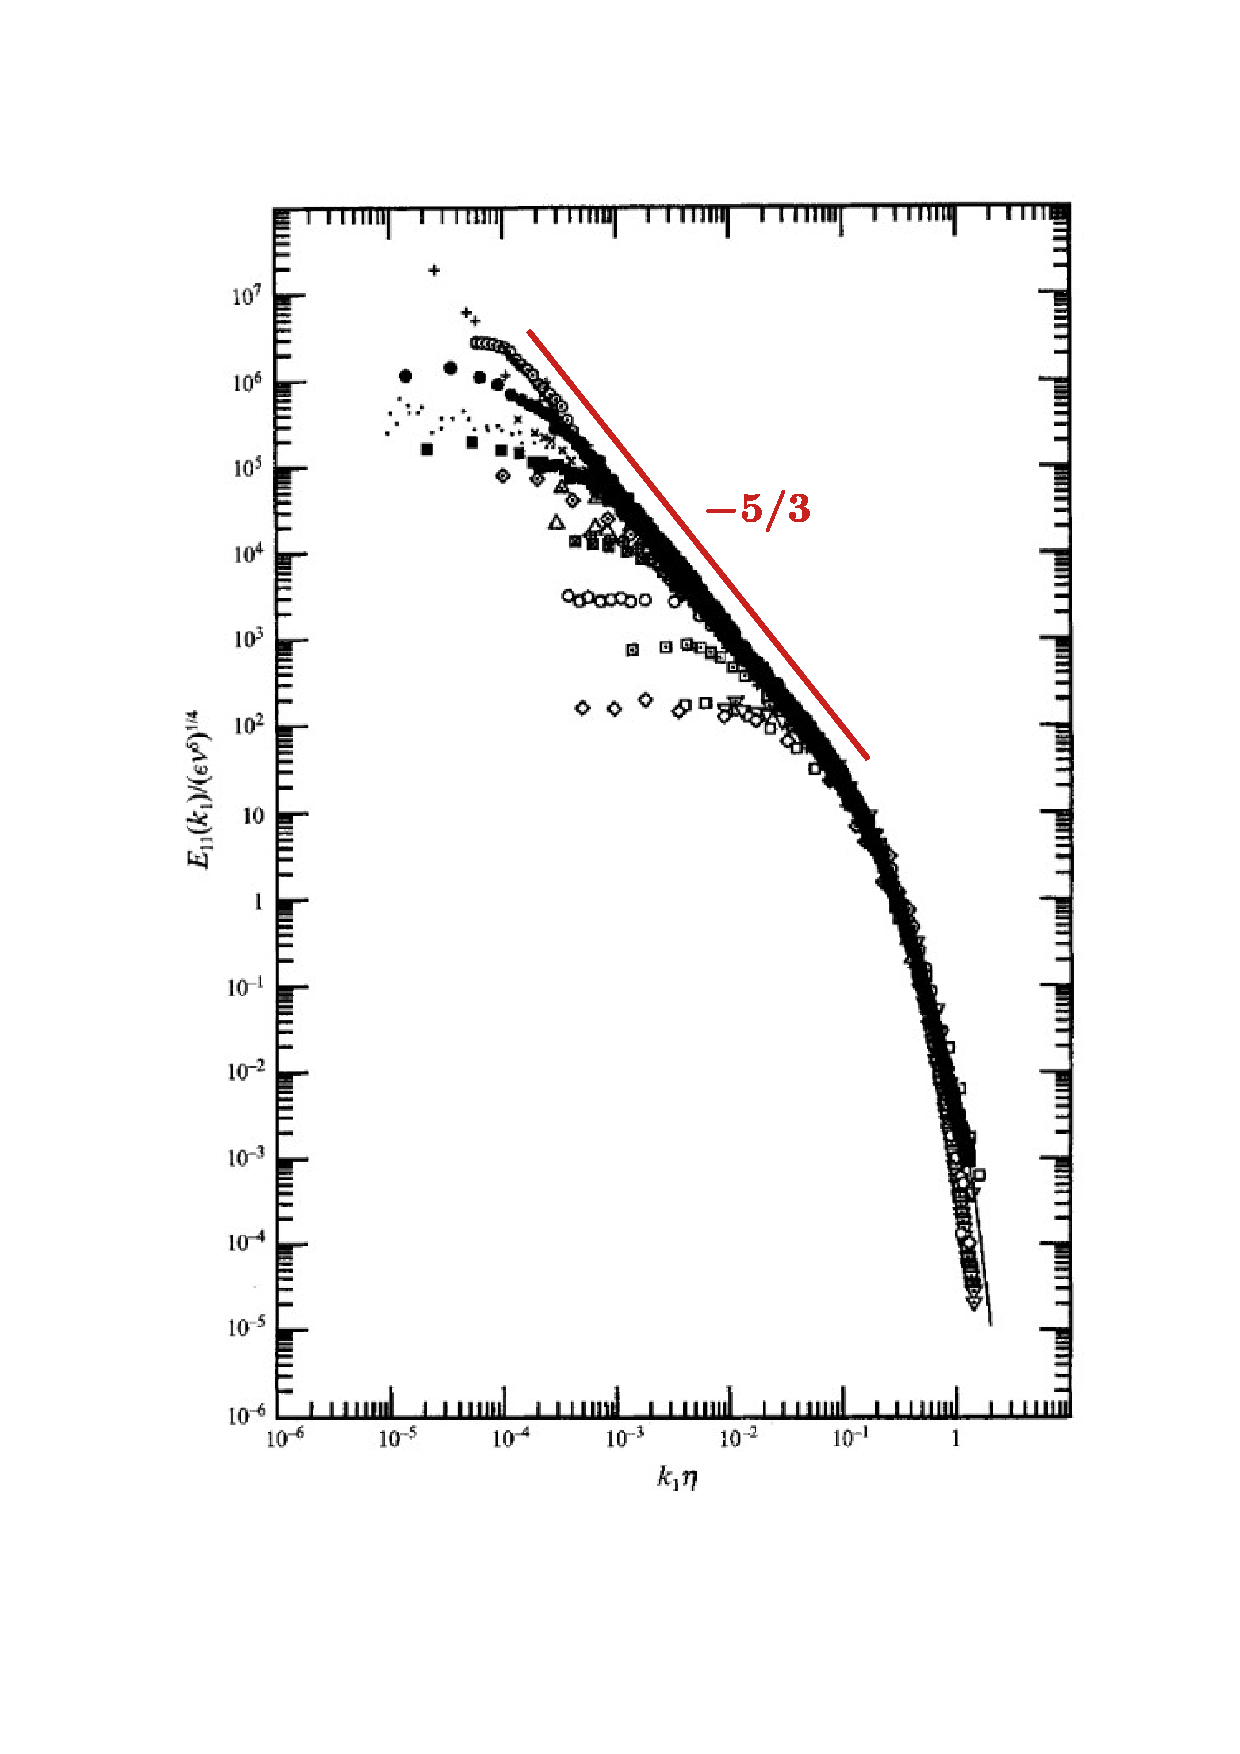
\includegraphics[width=0.8\linewidth,trim=1cm 4cm 1cm 3cm, clip=true]{./Part_0/images/spectre_kolmogorov}
\cprotect\caption{Compilations de spectres obtenus dans diverses expériences de laboratoire. Tous ces spectres sont en accord avec la pente en $-5/3$ prédite grâce à la théorie de Kolmogorov. Crédits : [\cite{saddoughi_local_1994}]. }
\label{fig:spec_kolmo}
\end{figure}
La forme $E(k) = C k^{\gamma}$ avec $C$ et $\gamma$ constants, qui s'écrit  en représentation logarithmique $\log E(k) = \gamma \log k + C $, est une loi d'échelle. Dans un système physique, une loi d'échelle ne va apparaître que sur une gamme d'échelle dédiée, limitée par la taille du système et l'émergence de phénomènes diffusifs à petites échelles, c'est à dire petits $\ell$ ou grand $k$. Ici, cette gamme est la zone de validité de la loi de Kolmogorov : la zone inertielle. 

Cette définition spectrale de la zone inertielle turbulente, telle que le spectre affiche une loi d'échelle en $-5/3$, n'est pas aussi contraignante que la définition statistique via un taux $\varepsilon$ constant. En effet, le système vérifiera plus facilement la définition spectrale que la définition statistique car $E(k)$ est d'ordre 2 ($\propto (\delta v)^2$ et positif) alors que $\varepsilon$ est d'ordre 3 ($\propto (\delta v)^3$ et signé). Autrement dit, observer une pente $-5/3$ de type Kolmogorov ne sera pas forcément synonyme d'un régime de turbulence complètement développée définie par l'existence d'une zone inertielle telle que $\varepsilon$ constant. 

\section{Synthèse des hypothèses de Kolmogorov et de la description de la cascade turbulente via des lois exactes}
\label{synt-01}
\fcolorbox{blue}{white}{\begin{minipage}[c]{\linewidth}
\paragraph{Taux énergétiques échelles-dépendants : }
\begin{itemize}
    \item Taux de cascade (transfert non linéaire entre les échelles) : $\varepsilon_{NL}(\boldsymbol{\ell})$
    \item Taux d'injection (forçage) : $\varepsilon_{F}(\boldsymbol{\ell})$
    \item Taux de dissipation : $\varepsilon_{D}(\boldsymbol{\ell})$
\end{itemize}

\paragraph{Loi zéroième ou anomalie dissipative : } $\varepsilon_{D}(\boldsymbol{\ell}= 0) \xrightarrow[\nu \rightarrow 0]{} - \varepsilon \neq 0$. $\varepsilon$ correspond au taux de dissipation turbulent.

\paragraph{Méthode d'obtention d'une loi exacte : }
\begin{itemize}
    \item Dériver l'évolution temporelle d'une fonction de corrélation $\mathcal{R}$ entre deux points indépendants $\mathbf{x}$ et $\mathbf{x'}$ séparés de l'échelle $\boldsymbol{\ell}$, 
    \item Prendre en compte l'hypothèse d'homogénéité statistique $\Rightarrow$ Loi exacte de type \acs{KHM}
    \item Appliquer les hypothèses de Kolmogorov de stationarité statistique et séparation d'échelle $\Rightarrow$ Loi exacte de type \acs{K41}
\end{itemize}

\paragraph{Propriété liée à l'hypothèse d'homogénéité statistique : } 
\begin{equation*}
    \Rightarrow \nabla_{\boldsymbol{\ell}}\left<.\right> = \left<\nabla' .\right> = - \left<\nabla . \right>
\end{equation*}

\paragraph{Propriété liée à l'hypothèse de stationnarité statistique : } $\Rightarrow \partial_t \left<.\right> = 0$.

\paragraph{Hypothèse de séparation d'échelle : } Séparation des gammes d'échelles d'injection/forçage, de cascade/inertielles, et de dissipation/chauffage permise par la loi zéroième. $\Rightarrow  \varepsilon_{NL}(0 \ll \boldsymbol{\ell} \ll \boldsymbol{\ell_F} ) = - \varepsilon_{F}(\boldsymbol{\ell} \ll \boldsymbol{\ell_F} ) = \varepsilon_{D}(\boldsymbol{\ell}=0) = - \varepsilon$.

\paragraph{Loi exacte de type \acs{KHM} : } $\partial_t \mathcal{R} = \varepsilon_{NL} + \varepsilon_{F} + \varepsilon_{D}$

\paragraph{Loi exacte de type \acs{K41} : } $\varepsilon = -\varepsilon_{NL}$

\end{minipage}}
